\documentclass[conference,10pt]{IEEEtran}
%\documentclass[conference,draft,onecolumn]{IEEEtran}
% useful packages, copy and paste from diff sources

%\usepackage[italian]{babel}
\usepackage[english]{babel}
\usepackage[T1]{fontenc}
\usepackage{cite,url,color} % Citation numbers being automatically sorted and properly "compressed/ranged".
\usepackage{graphics,amsfonts}
\usepackage{epstopdf}
\usepackage[pdftex]{graphicx}
\usepackage[cmex10]{amsmath}
% Also, note that the amsmath package sets \interdisplaylinepenalty to 10000
% thus preventing page breaks from occurring within multiline equations. Use:
\interdisplaylinepenalty=2500
% after loading amsmath to restore such page breaks as IEEEtran.cls normally does.
\usepackage[utf8]{inputenc}
% Useful for displaying quotations
%\usepackage{csquotes}
% Compact lists
%\let\labelindent\relax
\usepackage{enumitem}
\usepackage{multirow}
\usepackage{textcomp}

%tikz figures
\usepackage{tikz}
\usetikzlibrary{automata,positioning,chains,shapes,arrows}
\usepackage{pgfplots}
\usetikzlibrary{plotmarks}
\newlength\fheight
\newlength\fwidth
\pgfplotsset{compat=newest}
\pgfplotsset{plot coordinates/math parser=false}

\usepackage{array}
% http://www.ctan.org/tex-archive/macros/latex/required/tools/
%\usepackage{mdwmath}
%\usepackage{mdwtab}
%mdwtab.sty	-- A complete ground-up rewrite of LaTeX's `tabular' and  `array' environments.  Has lots of advantages over
%		   the standard version, and over the version in `array.sty'.
% *** SUBFIGURE PACKAGES ***
%\usepackage[tight,footnotesize]{subfigure}
\usepackage{subfig}

\usepackage[top=1.5cm, bottom=2cm, right=1.6cm,left=1.6cm]{geometry}
\usepackage{indentfirst}

\usepackage{times}
% make sections titles smaller to save space
%\usepackage{sectsty}
%\sectionfont{\large}
% enable the use of 'compactitem', a smaller 'itemize'
%\usepackage{paralist}

% MP
% to split equations using dmath env
\usepackage{breqn}
% nice rules in tables
\usepackage{booktabs}

%\setlength\parindent{0pt}
\linespread{1}

% MC
\newcommand{\MC}[1]{\textit{\color{red}MC says: #1}}
\newcommand{\AZ}[1]{\textit{\color{blue}AZ says: #1}}
\newcommand{\MP}[1]{\textit{\color{green}MP says: #1}}

\usepackage{placeins}


%%%%%%%%%%%%%%%%%%%%%%%%%%%%%%%%%%%%%%%%%%
\begin{document}
%%%%%%%%%%%%%%%%%%%%%%%%%%%%%%%%%%%%%%%%%%
\title{Applicazione della Logica Fuzzy\\ in un Sistema di Irrigazione}

\author{\IEEEauthorblockN{Giuseppe Ravagnani, Marco Sansoni}
\IEEEauthorblockA{Laurea Magistrale in Ingegneria Informatica - Sistemi Intelligenti\\Dipartimento di Ingegneria dell'Informazione, Università di Padova
}}

\maketitle

\begin{abstract}
Un sistema di irrigazione intelligente ottimizza l'acqua necessaria per il corretto sostentamento della pianta mediante l'impiego di sensori e l'utilizzo della logica fuzzy.
In base all'umidità del terreno e alla temperatura dell'aria un sistema a feedback richiederebbe un considerevole impiego di tempo per ottenere risultati soddisfacenti; al contempo la logica fuzzy risulta più flessibile alle esigenze di una pianta in quanto simula l'opera umana, garantendo un sistema più robusto ad eventi non previsti, con un minor dispendio d'acqua. Nel seguito forniremo un valido modello di assorbimento che regola  l'acqua che viene fornita tramite precipitazioni, quella assorbita dalla pianta in fase di evapotraspirazione, e inoltre anche quella evaporata dal terreno. Su questo modello astratto impiegheremo la logica fuzzy per determinare in maniera intelligente il fabbisogno vitale di acqua della pianta. Si giustificherà infine l'effettivo vantaggio legato a questo approccio fuzzy.
\end{abstract}

%%%%%%%%%%%%%%%%%%%%%%%%%%%%%%%%%%%%%%%%%
\section{Introduzione}\label{sec:intro}
%%%%%%%%%%%%%%%%%%%%%%%%%%%%%%%%%%%%%%%%%
L'acqua è la componente chiave di tutte le forme di vita conosciute sulla Terra, è una risorsa naturale primaria che non deve andare sprecata. In agricoltura la mancanza comporta l'inevitabile secchezza e morte della pianta; d'altro canto un utilizzo troppo abbondante comporta problematiche come una crescita impropria delle colture. La chiave nell'irrigazione è fornire un corretto bilanciamento della pianta con un ridotto uso d'acqua \cite{2}.\\
L'idea di un sistema automatizzato di irrigazione non è nuova, si sono infatti sviluppati, fino al giorno d'oggi, differenti sistemi di irrigazione automatica. Sistemi efficienti di irrigazione automatica, che riescono a fornire la quantità d'acqua perfetta per la crescita della pianta, non esistono, risolverebbero altrimenti ogni problema relativo allo spreco d'acqua \cite{4}.\\
Al giorno d'oggi sul mercato possiamo già trovare differenti sistemi pensati ad automatizzare impianti di irrigazione.
Si trovano, infatti, centraline che regolano solamente l'inizio e la fine dell'irrigazione, senza effettuare una verifica dello stato di salute della pianta e delle sue effettive necessità \cite{1}.\\
Possiamo però trovare anche modelli più elaborati che provvedono dinamicamente a fissare la quantità d'acqua da erogare alla pianta in base ai valori misurati nell'ambiente.\\
Quest'ultimo metodo è però molto sensibile alle piccole variazioni, sono composti infatti da rudimentali modelli matematici che determinano l'acqua in funzione dei valori presenti istante per istante \cite{3}. \\
Il sistema basato su logica fuzzy elabora l'acqua in modo simile al pensiero umano, più resistente e robusto alle variazioni non ipotizzate preventivamente. \\
La motivazione della ricerca è lo sviluppo di un modello più efficiente di irrigazione riducendo al minimo l'intervento umano sfruttando la logica fuzzy.
L'idea della logica fuzzy è stata proposta inizialmente da L. A. Zadeh in una pubblicazione pubblicata nel 1968 e nel 1972, descritta poi più nel dettaglio nel 1973.
Un suo ampio utilizzo è dovuto all'abilità della logica di modellare, in modo preciso, l'abilità della mente umana di prendere decisioni razionali in un ambiente incerto e impreciso \cite{9}.\\
Una sua applicazione nel campo dell'irrigazione viene descritta nella seguente trattazione. \\ Si sfruttano i vantaggi ad essa legati per prendere decisioni relative a quanto far durare il periodo di innaffiamento in base ad informazioni fornite dalla pianta come l'umidità del terreno, e dati ricavati dall'ambiente circostante quali temperatura e umidità dell'aria.\\
Nella nostra trattazione forniremo una implementazione significativa di un sistema di irrigazione mediante logica fuzzy. \\
Per testare i valori e l'effettiva bontà del sistema, è stato necessario introdurre un modello realistico di come l'umidità e la quantità d'acqua nel terreno variano durante il tempo.\\
Sono stati utilizzati dati reali come temperatura, umidità, ma anche valori che influenzano attivamente il bisogno d'acqua della pianta come le precipitazioni \cite{7}.\\ Si è inoltre considerato la quantità d'acqua assorbita dalla pianta per le sue funzioni vitali.\\
successivamente sono state definite tutte le varie regole di inferenza necessarie per determinare, mediante logica fuzzy, il quantitativo necessario di acqua per minimizzare lo spreco d'acqua garantendo comunque la salute della pianta.\\
Dall'andamento finale dei risultati ottenuti si può constatare, come il modello presentato, mediante l'utilizzo di logica fuzzy, restituisce risultati convincenti, garantendo uno stato di salute ottimale della pianta con un minimo utilizzo d'acqua.

%%%%%%%%%%%%%%%%%%%%%%%%%%%%%%%%%%%%%%%%%%%%
\section{Stato dell'arte}\label{sec:sota}
%%%%%%%%%%%%%%%%%%%%%%%%%%%%%%%%%%%%%%%%%%%%
Gli attuali sistemi di irrigazione automatizzata presenti sul mercato differiscono in base allo scarso e all'eccessivo uso di sensori che forniscono una panoramica sull'ambiente circostante.\\
Come accennato brevemente nell'introduzione di questo documento, le classi principali dei modelli di irrigazione autonoma presenti sul mercato si possono classificare in due macro categorie:

\begin{itemize}
	\item Controllori ad anello aperto: sono basati su predefiniti sistemi di controllo che non richiedono l'utilizzo di un feedback dall'ambiente. I più semplici controllori presenti sul mercato operano infatti nel seguente modo. L'utente imposta l'orario iniziale e quello finale, eventuali periodi di pausa e il tempo di irrigazione.\\ 
	Sono presenti parametri fissati inizialmente che continuano a rimanere validi per tutta la sessione come quanto spesso bisogna ripetere l'operazione di irrigazione e per quanto tempo, e la quantità d'acqua che sarà utilizzata nel processo \cite{1}.\\
	\item Controllori ad anello chiuso o Controllori a feedback: rientrano in questa categoria tutti i principali controllori che si basano su una combinazione di parametri impostati inizialmente e un riscontro sui valori analizzati mediante sensori. \\
	Sono presenti numerosi fattori che possono influenzare la decisione relativa alla quantità d'acqua necessaria. Alcuni sono fissati durante la sessione e derivano da caratteristiche intrinseche della pianta, altri vengono analizzati durante la sessione.\\
	Il sistema in catena chiusa analizza questi parametri fornendo in uscita risultati come:
	\begin{itemize}
		\item La durata della sessione di irrigazione
		\item La periodicità con cui l'operazione si deve ripetere
		\item La quantità di acqua che viene utilizzata nella sessione corrente
	\end{itemize}
	Questi controllori presentano punti di criticità quando si va ad analizzare valori sui consumi effettivi di acqua. Presentano inoltre problemi quando accidentalmente un parametro non viene letto correttamente oppure quando si presentano dati non previsti.\\
	In questi casi il controllore fornisce come uscita quantità d'acqua non previste, che vanno ad inficiare sullo stato di salute della pianta.\\ Il controllore ad anello chiuso è quindi molto sensibile ad ogni variazione sui parametri in esame \cite{1}.
	\newline
\end{itemize}
Il bilancio idrico della pianta è un argomento molto sviluppato nel settore ambientale, e sono presenti in letteratura modelli, che presentano differenti gradi di accuratezza, che vanno a spiegare dettagliatamente il fabbisogno di una pianta \cite{11}.\\
Aspetto fondamentale per andare a capire il modello è l'evapotraspirazione, ovvero "la somma della quantità d’acqua persa dal suolo per evaporazione e dalle piante per traspirazione" \cite{6}. \\
L'evapotraspirazione raccoglie quindi il bilancio idrico relativo all'acqua in uscita dal modello, assorbita o evaporata.

%%%%%%%%%%%%%%%%%%%%%%%%%%%%%%%%%%%%%%
\section{Contributo}\label{sec:symo}
%%%%%%%%%%%%%%%%%%%%%%%%%%%%%%%%%%%%%%
Andremo ora ad analizzare l'introduzione della logica fuzzy in un sistema di irrigazione. Verrà proposto un esempio con dati significativi che determina in maniera autonoma il quantitativo di acqua necessario per il fabbisogno della pianta.
Inizialmente abbiamo introdotto un modello per andare ad analizzare il bilancio idrico della pianta.\\
L'introduzione del modello deriva dalla necessità di fornire un esempio significativo con dati reali dell'efficacia della logica fuzzy. Si usa quindi un sistema reale del bilancio idrico di una pianta che definisce ad ogni istante l'umidità presente nel terreno, parametro chiave per l'irrigazione.\\
Forniremo successivamente una implementazione mediante MATLAB, necessaria per andare a sperimentare realmente i benefici legati a questo modello.\\
Nell'implementazione i valori presenti, di temperatura, umidità dell'aria e precipitazioni, sono forniti da dati reali provenienti da un data set reperito online \cite{7}. \\
Alternativamente a quanto fatto si potrebbero andare ad analizzare dati reali provenienti da un sensore che misura di volta in volta l'umidità del terreno.

%%%%%%%%%%%%%%%%%%%%%%%%%%%%%%%%%%%%%%
\subsection{Descrizione del Modello}\label{sec:symo}
%%%%%%%%%%%%%%%%%%%%%%%%%%%%%%%%%%%%%%
Il fabbisogno di acqua di una pianta è legato all'ambiente in cui è cresciuta, ma anche ad aspetti intrinsechi della pianta, dalla sua tipologia (sempreverde, grassa, \dots), così come anche al differente periodo dell'anno \cite{3}.
Come ipotesi conservativa, facilmente modificabile a seconda della pianta oggetto dell'irrigazione, abbiamo supposto come effettuiamo il controllo ogni 6 ore, e a seconda del valore fornito dalla logica fuzzy provvederemo o meno all'irrigazione.\\
Abbiamo ipotizzato un sistema di irrigazione del tipo a goccia, che fornisce un valore di acuqa diluito nel tempo che consente un migliore assorbimento della pianta, altrimenti si rischierebbe che una quantità d'acqua sia sprecata o non completamente assorbita dal suolo.\\
Dopo ogni intervallo di 6 ore sarà quindi presente un differente valore d'acqua nel suolo.\\ Possiamo quindi assumere valida la seguente formula che regola il bilancio idrico della pianta.
\begin{equation*}
\frac{\Delta A}{\Delta t} = P + I - ET_c
\end{equation*}
dove:
\begin{itemize}
	\item $\frac{\Delta A}{\Delta t}$ è la differenza di acqua nel suolo nell'intervallo di tempo scelto precedentemente $[mm/h]$
	\item $P$ è la quantità delle precipitazioni $[mm/h]$ 
	\item $I$ è la quantità d'acqua fornita durante la fase di irrigazione al controllo precedente $[mm/h]$
	\item $ET_c$ è la somma della quantità d'acqua assorbita per traspirazione dalla specifica pianta in esame e l'evaporazione dell'acqua dal suolo $[mm/h]$
	\newline
\end{itemize}
Notiamo come le quantità d'acqua coinvolte nel processo sono le precipitazioni avvenute nelle precedenti 6 ore trascorse, e l'acqua fornita dal sistema di irrigazione nella fase precedente, che risultano parte attiva del bilancio idrico nel successivo controllo.\\
L'ultimo parametro merita una digressione: l'evapotraspirazione infatti è la somma della quantità d’acqua persa dal suolo per evaporazione e dalle piante per traspirazione, corrisponde a tutta l'acqua che nel bilancio idrico deve essere sottratta \cite{6}. \\
Per poter definire più nel dettaglio l'evapotraspirazione della specifica coltura dobbiamo prima definire:
\begin{itemize}
	\item $ET_o$ rappresenta per convenzione il “riferimento” per poter stimare i consumi idrici di tutte le
	altre colture, in qualunque condizione ambientale e a qualunque stadio vegetativo esse si trovino
	\item $K_c$ è un coefficiente colturale, specifico per ogni cultura
\end{itemize}
Una volta definito, la seguente formula fornisce il valore esatto di $ET_c$.
\begin{equation*}
ET_c = K_c \cdot ET_o
\end{equation*}
In letteratura sono presenti differenti versioni per stimare il valore di $ET_o$, nel nostro modello utilizziamo la formula di Valiantzas \cite{8}. \\
\begin{equation*}
\begin{split}
ET_o &\approx 0.0393R_s\sqrt{T_a + 9.5} -\\ &-0.019R_s^{0.6}\Phi^{0.15}+0.048(T_a+20)(1-\frac{R_h}{100})
\end{split}
\end{equation*} 
dove:
\begin{itemize}
	\item $R_s$ Radiazione solare $[MJ/m^2/day]$
	\item $T_a$ Temperatura media dell'aria giornaliera $[°C]$
	\item $\Phi$ Latitudine del sito $[rad]$
	\item $R_h$ Umidità dell'aria $[\%]$
	\newline
\end{itemize}
Per una migliore comprensione risulta inevitabile notare le unità di riferimento delle formule sopra definite.
Si ha come il bilancio idrico della pianta contenga tutti i differenti valori espressi in $mm$.
\\Nella nostra trattazione, ad ogni analisi periodica, effettuata quindi ogni 6 ore, viene aggiunta questo bilancio all'umidità del suolo calcolata precedentemente. Come nostra convenzione abbiamo posto l'equivalenza 1 $mm$ = 1 \% dell'umidità, in quanto la stima risente del graduale tempo di assorbimento del suolo, ma una spiegazione più approfondita esula dell'obiettivo della trattazione.
\\ Così facendo riusciamo a determinare in maniera abbastanza accurata l'umidità presente nel terreno al momento della verifica, in modo da poter fornire il valore trovato alla logica fuzzy che ne determinerà poi l'acqua da fornire. \\
Il valore restituito dalla logica fuzzy, corrisponderà successivamente al parametro $irrigazione$, da andare a considerare nel bilancio idrico della pianta per il successivo controllo.\\
Possiamo descrivere tutti i passaggi analizzati precedentemente nel diagramma di flusso nella Figure 1.\vspace*{0.1 cm}
\begin{figure}[ht]
	\centering
	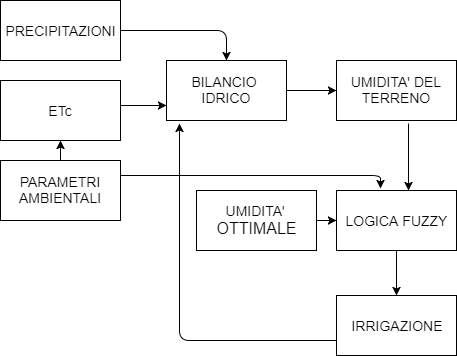
\includegraphics[width=0.8\linewidth]{images/flusso.png}
	\caption{Diagramma di flusso del sistema}
	\label{fig:flusso}
\end{figure}

Nel diagramma di flusso troviamo un ultimo blocco dello schema precedente che deve essere ancora trattato approfonditamente, ovvero il valore di umidità ottimale da fornire alla pianta.\\
Definiamo inizialmente il concetto del massimo valore di svuotamento (MAD dall'inglese Management Allowed Depletion).
Si tratta del minimo valore di umidità del terreno che può essere sostenuto dalla pianta, per evitare di ricadere in una zona di stress.
Questo è il punto esatto nel quale deve iniziare il processo di irrigazione per evitare che lo stress influenzi la crescita ottimale della pianta \cite{5}.\\ 
Analogamente al valore minimo troviamo anche un valore massimo accettato di umidità del terreno, il cui eccesso porta il suolo in un regime di saturazione, meno critico rispetto alla secchezza del terreno, ma comunque la quantità d'acqua presente risulta eccessiva per il benessere della pianta. Questo ci fornisce un intervallo ottimo di valori di umidità, cui desideriamo mantenerci in tutto l'arco del processo di irrigazione.\\
Il valore non è universalmente definito per ogni tipo di condizione ma si differenzia principalmente rispetto al tipo di terreno su cui viene effettuata l'irrigazione. Per fare un esempio, su un terreno sabbioso, è sufficiente una piccola percentuale di umidità del terreno per il benessere della pianta, al contrario il valore si alza notevolmente in caso di un terreno argilloso \cite{5}. \\
Nella nostra implementazione supponiamo una pianta posta in un terreno di tipo argilloso.\\ Dalla letteratura ricaviamo i valori ottimali di umidità del terreno per evitare la zona di stress e di saturazione, come mostrato in Figure 2.\vspace*{0.1 cm}
\begin{figure}[ht]
	\centering
	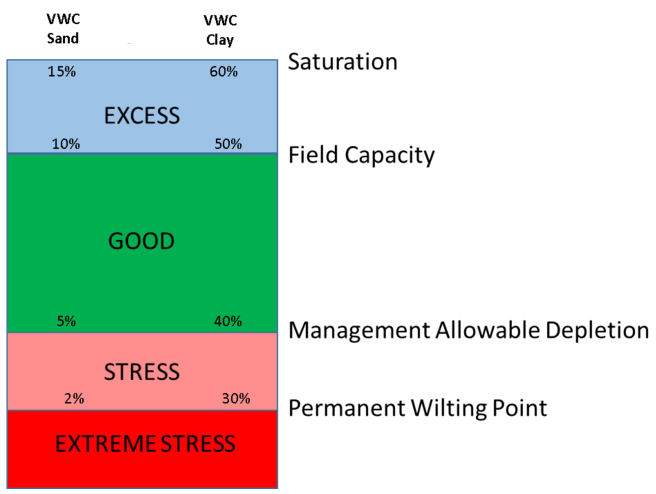
\includegraphics[width=0.8\linewidth]{images/SoilMoistureTerms.png}
	\caption{Umidità del terreno}
	\label{fig:MAD}
\end{figure}
\\Siamo andati a definire e analizzare tutti gli aspetti fondamentali legati all'ambiente sufficienti per poter fornire alla pianta l'ottimo valore di irrigazione.\\
Nella successiva sezione andremo a analizzare la logica che regola il meccanismo di irrigazione, e la nostra implementazione del modello.

%%%%%%%%%%%%%%%%%%%%%%%%%%%%%%%%%%%%%%
\subsection{Implementazione della Logica Fuzzy}\label{sec:symo}
%%%%%%%%%%%%%%%%%%%%%%%%%%%%%%%%%%%%%%
Il meccanismo fondamentale che regola il sistema intelligenti di irrigazione è costituito dalla logica fuzzy.\\
Dobbiamo quindi andare a determinare ogni parametro che fornisce lo schema generale del funzionamento, come descritto in Figure 3.
\begin{figure}[ht]
	\centering
	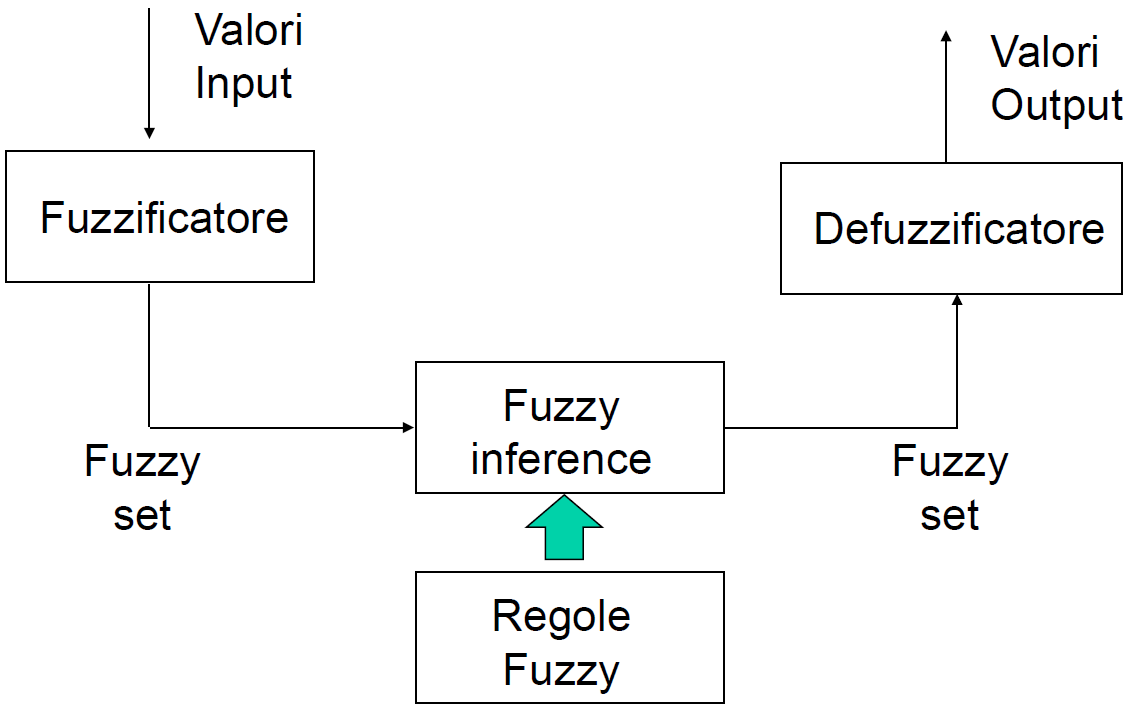
\includegraphics[width=0.8\linewidth]{images/schemafuzzy.png}
	\caption{Schema Logica Fuzzy}
	\label{fig:MAD}
\end{figure}
\\Come primo valore da determinare bisogna conoscere quali sono i valori necessari di input per poter effettuare la scelta migliore. Sarà infatti grazie a quei parametri, che verrà poi ponderata la scelta in uscita.\\
Valori fondamentali risultano essere la temperatura, l'umidità del terreno e dell'aria, valori che andremo successivamente a definire nei fuzzy sets.\\
L'ultimo valore di input che andremo ad utilizzare sarà un valore legato all'umidità del terreno, dove considereremo però la differenza tra l'umidità presente e l'umidità ottima. Avremo quindi l'ultimo parametro definito da:\\
\begin{equation*}
\begin{split}
Differenza = Umidit\grave{a}\text{ }Misurata-Umidit\grave{a}\text{ }Ottima
\end{split}
\end{equation*}  
In questo modo i possibili valori ottenuti indicano la quantità d'acqua da andare a somministrare alla pianta in caso di valori fortemente negativi si è infatti presenti nella zona di stress della pianta.\\
Con questi parametri in input, tramite fuzzificazione, abbiamo definito i relativi fuzzy set, come mostrato in Figure 4, Figure 5 e Figure 6.
\begin{figure}[ht]
	\centering
	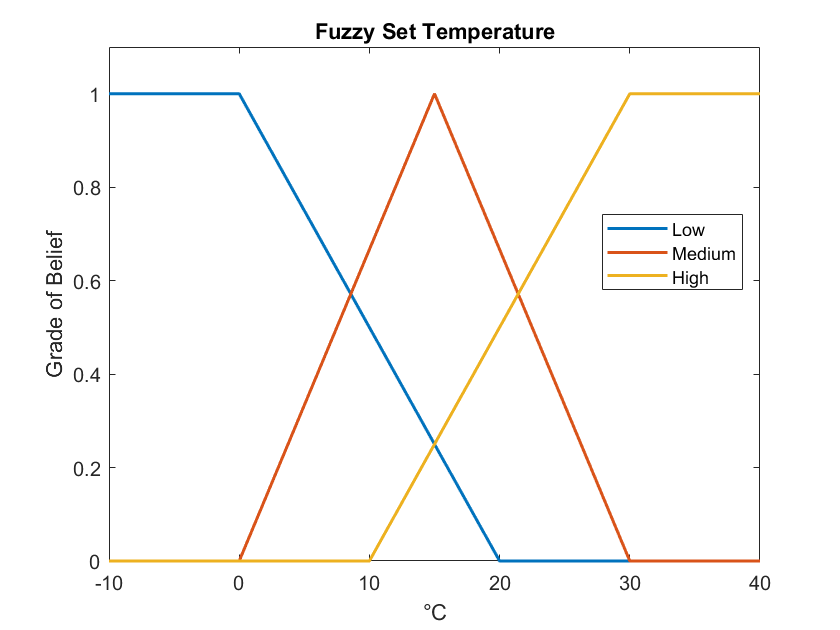
\includegraphics[width=1\linewidth]{images/temp_fs.png}
	\caption{Fuzzy Set Temperatura}
	\label{fig:MAD}
\end{figure}\\
\begin{figure}[ht]
	\centering
	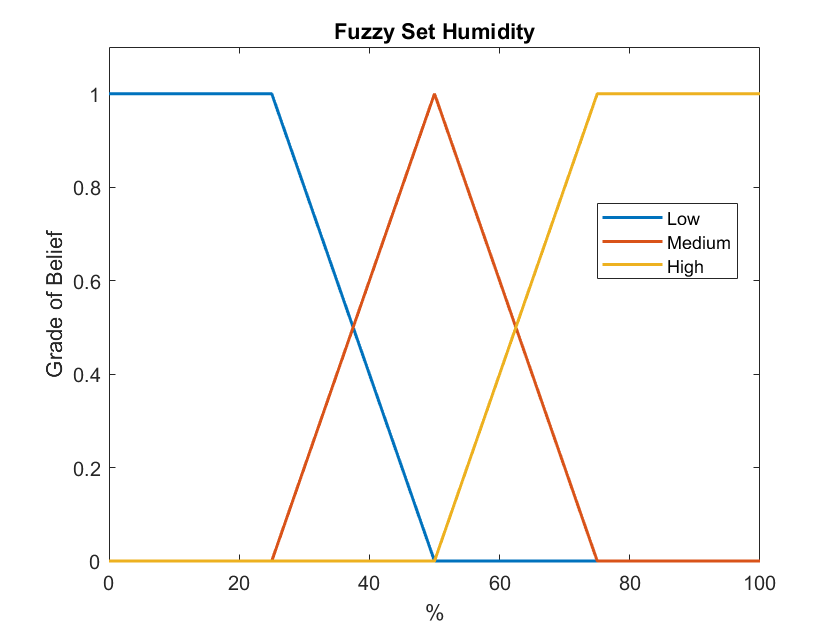
\includegraphics[width=1\linewidth]{images/humi_fs.png}
	\caption{Fuzzy Set Umidità}
	\label{fig:MAD}
\end{figure}\\
\begin{figure}[ht]
	\centering
	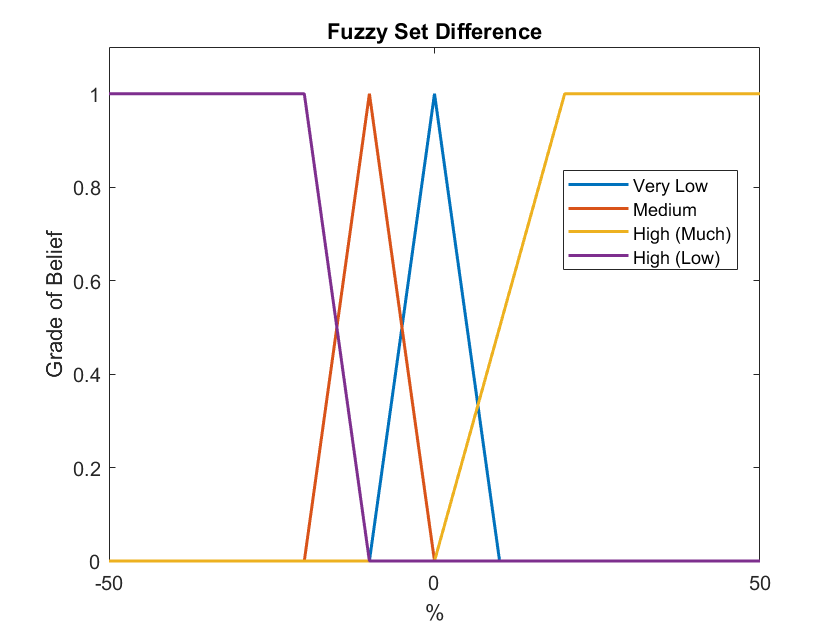
\includegraphics[width=1\linewidth]{images/diff_fs.png}
	\caption{Fuzzy Set Differenza Umidità terreno}
	\label{fig:MAD}
\end{figure}
\newpage
Una volta definiti i Fuzzy Sets, dobbiamo definire le regole di inferenza che utilizzeremo nel seguito che andranno a regolare le logiche di irrigazione.\\
Per una trattazione generale definiamo ogni variabile in input come $x_i$, dove $i$ rappresenta l'indice della variabile di controllo.
Nei grafici precedenti possiamo determinare per ogni variabile in input dei differenti fuzzy sets (Alta, media, bassa, \dots). Per facilità di trattazione definiamo questi specifici sottoinsiemi come $A_{ij}$ dove indichiamo l'etichetta j-esima associata alla variabile in input i-esima. Ad esempio, considerando la variabile $x_1$, i differenti valori delle $n$ etichette, saranno indicati con $A_{1j}$.\\
Nel nostro caso in esame sono presenti tre differenti valori della variabile in input, e quindi le regole di inferenza coprono tutti i differenti casi possibili, dove ognuna ritorna un scelta per il sistema di irrigazione.\newpage
Ogni regola fuzzy presenta una struttura del tipo:\\
\begin{equation*}
\begin{split}
&IF\;x_1\;is\;A_{11}\;AND\;x_2\;is\;A_{21}\;AND\;x_3\;is\;A_{31}\\
&OR \\
&IF\;x_1\;is\;A_{12}\;AND\;x_2\;is\;A_{22}\;AND\;x_3\;is\;A_{32}\\
&OR\;\dots\\
&IF\;x_1\;is\;A_{1n}\;AND\;x_2\;is\;A_{2n}\;AND\;x_3\;is\;A_{3n}\\
&THEN\text{ l'azione da prendere è }Y.
\end{split}
\end{equation*}
\\Per fornire un esempio concreto della nostra implementazione si sono scritte, ad esempio, le seguenti regole di inferenza:\\
\begin{equation*}
\begin{split}
&IF\;T\;is\;HIGH\;AND\;D\;is\;HIGH(LOW)\;AND\\\;&H\;is\;LOW\\
&OR \\
&IF\;T\;is\;HIGH\;AND\;D\;is\;HIGH(LOW)\;AND\\\;&H\;is\;MEDIUM\\
&OR\;\\
&IF\;T\;is\;HIGH\;AND\;D\;is\;HIGH(LOW)\;AND\\\;&H\;is\;HIGH\\
&THEN\text{ la quantità d'acqua è }tanta.
\end{split}
\end{equation*}
\\Nel nostro modello sono state definite, in accordo con i grafici precedenti relativi ai fuzzy sets, 3 differenti valori possibili per temperatura e umidità, mentre sono 4 i differenti valori che può assumere l'output della differenza. Sono quindi presenti tutte le possibili 36 combinazione. Nel caso particolare appena proposto, viene evidenziato come in caso di elevate temperature e differenze di umidità, indipendentemente dall'umidità, viene fornito dal sistema un valore di acqua elevato.
\\Tutte le altre regole di inferenza, così come i valori associati all'output sulla quantità d'acqua fornita dall'impianto di irrigazione, sono stati progettati come utilizzabili in una reale applicazione, come agirebbe quindi la mente umana.\\
Restano da determinare ora i valori di verità associati ai differenti output. In accordo con le regole di inferenza definite precedentemnete e con la logica fornita da Lukasievicz (Logic L1) \cite{10}, l'istruzione $AND$ viene risolta con un $min$ mentre l'istruzione $OR$ viene risolta con $max$.\\
Sfruttando questo otteniamo il valore di verità associato ad $Y$, come:\\
\begin{equation*}
\mu_Y= \bigcup\limits_{j=1}^{n} \left[ \bigcap\limits_{i=1}^{3} \mu_{A_{ij}}\left(x_i \right)  \right] 
\end{equation*}
\\Il processo prevede infine il passaggio di defuzzificazione.\\
Considerando l'azione da intraprendere $Y$ come un insieme dei possibili valori da dare al sistema di irrigazione, contenenti la quantità d'acqua in mm da fornire all'impianto.
Indichiamo con $Y_i$ tutti i valori possibili delle quantità d'acqua associate all'output. Resta quindi da calcolare il valore esatto $I$ d'acqua come media ponderata dei valori di verità.
La formula finale è quindi:\\
\begin{equation*}
I=\dfrac{\sum \mu(Y_i)*Y_i}{\sum \mu (Y_i)}
\end{equation*} 
\\Nella nostra implementazione viene utilizzata questa logica appunto per trovare il valore d'acqua ottimale. Riportiamo nella tabella sottostante un esempio di applicazione in un istante generico.\\ Troviamo infatti nella Table I sottostante i valori misurati delle tre differenti grandezze in input al problema, con associata per ogni grandezza il valore di verità di ogni label che caratterizza la variabile nel fuzzy set.


\begin{table}[ht]
	\centering
	\caption{Valori in input con grado di verità}
	{\renewcommand\arraystretch{1.7}
	\begin{tabular}{|l|l|}\hline
		\multirow{3}{*}{Temperatura: 29.1 °C}  & $\mu_{L}$ = 0 \\ \cline{2-2} &  $\mu_{M}$ = 0.06 \\ \cline{2-2}  &  $\mu_{H}$ = 0.9550 \\ \cline{2-2}
		\hline
		\multirow{3}{*}{Umidità: 78 $\%$}  & $\mu_{L}$ = 0 \\ \cline{2-2} &  $\mu_{M}$ = 0 \\ \cline{2-2}  &  $\mu_{H}$ = 1 \\ \cline{2-2}
		\hline
		\multirow{4}{*}{Differenza: 1.0556 $\%$}  & $\mu_{L}$ = 0.8944 \\ \cline{2-2} &  $\mu_{M}$ = 0 \\ \cline{2-2}  &  $\mu_{HM}$ = 0.0528 \\ \cline{2-2} &  $\mu_{HL}$ = 0 \\ \cline{2-2}
		\hline
	\end{tabular}}	
\end{table}
Nella Table II sottostante troviamo, invece, il valore di verità che caratterizzano l'output di uscita, ovvero un valore associato ad ogni etichetta del tipo "Tanta acqua".
Per ogni valore di output abbiamo associato un valore discreto come riportato nella tabella, tale parametro risulta necessario in fase di defuzzificazione.\\
\begin{table}[ht]
	\centering
	\caption{Valori di verità di irrigazione e quantità finale}
	{\renewcommand\arraystretch{1.7}
	\begin{tabular}{|l|l|}\hline
		Niente: 0 $mm$  & $\mu_{N}$ = 0.06 \\ \cline{2-2} 
		\hline
		Poca: 5 $mm$ & $\mu_{P}$ = 0.8944 \\ \cline{2-2} 
		\hline
		Abbastanza: 10 $mm$ & $\mu_{A}$ = 0 \\ \cline{2-2} 
		\hline
	    Tanta: 20 $mm$  & $\mu_{T}$ = 0  \\\cline{2-2} 
		\hline
		\multicolumn{2}{|c|}{Quantità d'acqua: 4.6857 $mm$} \\
		\hline		
	\end{tabular}}	
\end{table}



%%%%%%%%%%%%%%%%%%%%%%%%%%%%%%%%%%%%%%
\subsection{Implementazione nel mondo reale}\label{sec:symo}
%%%%%%%%%%%%%%%%%%%%%%%%%%%%%%%%%%%%%%
Merita una piccola riflessione come implementare il modello descritto precedentemente nel mondo reale, quando viene data una applicazione all'astrazione fornita da questa implementazione.\\
Nel nostro caso, non disponendo di una coltura e di una pianta dove effettuare la verifica abbiamo utilizzato dati proveniente da un dataset, relativa ad una zona paragonabile alla nostra città come clima. Abbiamo infatti ottenuto dati reali delle precipitazioni atmosferiche, temperatura e umidità dell'aria.\\
Nel nostro modello, non potendo ricavare online valori reali dell'umidità del terreno, abbiamo realizzato questo modello che descrive l'andamento dell'umidità del suolo per poter effettuare la simulazione.\\
Nella implementazione nel mondo reale risulta però inutile il modello precedente relativo all'umidità del suolo, in quanto basta prelevare dall'ambiente il valore cercato dell'umidità ogni 6 ore, nel momento del controllo, mediante l'utlizzo di un sensore.\\
Riassumendo i valori necessari da ottenere in tempo reale dal sistema attorno alla coltura per l'irrigazione sono la temperatura, l'umidità dell'aria e quella del terreno.
Il sensore provvede a fornire i valori al sistema in logica fuzzy, che analizzandoli mediante fuzzy set, provvederà poi a fornire il valore necessario di acqua. I seguenti passaggi saranno spiegati poi nel dettaglio nelle seguenti sezioni.


%%%%%%%%%%%%%%%%%%%%%%%%%%%%%%%%%%%%%%
\subsection{Modello di controllore in catena chiusa}\label{sec:symo}
%%%%%%%%%%%%%%%%%%%%%%%%%%%%%%%%%%%%%%
Per andare a notare i vantaggi ottenuti mediante l'uso della logica fuzzy è interessante andare a notare come variano i risultati in caso di implementazione di un modello alternativo. Per l'occasione abbiamo sviluppato un controllore in catena chiusa.\\
Come spiegato nella sezione relativa allo stato dell'arte, i controllori in catena chiusa sono una famiglia di sistemi di irrigazione automatica molto diffusi sul mercato, che determinano il valore di acqua da fornire alla pianta in base ad una funzione su determinati valori dell'ambiente ricavati medianti sensori.\\
Nel nostro esempio abbiamo implementato un rudimentale sistema con la seguente logica: viene fornito tramite l'impianto un valore di acqua costante ogni 24 ore, prima di fare ciò però viene eseguito un controllo sull'umidità presente nel terreno. Quando troviamo infatti un valore eccessivo non azioniamo l'impianto, e lo rimandiamo alla verifica successiva, senza eseguire l'irrigazione.
\begin{figure}[ht]
	\centering
	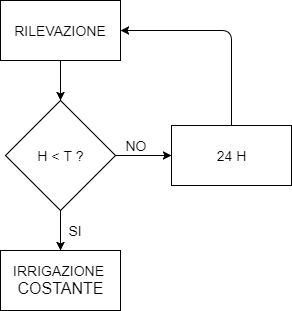
\includegraphics[width=0.6\linewidth]{images/ccc.png}
	\caption{Digramma a blocchi controllore in catena chiusa}
	\label{fig:MAD}
\end{figure}

In questo caso il valore di umidità ottima è lo stesso utilizzato per il sistema con logica fuzzy, ricavato dalla Figure 2; abbiamo quindi determinato, ancora una volta, come 50\% risulta il valore soglia, sopra al quale non viene fatta l'irrigazione.\\
L'idea del controllore in catena chiusa appena descritta, viene rappresentata nel diagramma a blocchi in Figure 7.\\
Nello schema la decisione è implementata mediante il controllore in catena chiusa, dove la funzione è determinata appunto dallo specifico confronto.


%%%%%%%%%%%%%%%%%%%%%%%%%%%%%%%%%%%%%%%%%%%%%%%
\section{Risultati}\label{sec:res}
%%%%%%%%%%%%%%%%%%%%%%%%%%%%%%%%%%%%%%%%%%%%%%%
Nella nostra simulazione abbiamo sviluppato il modello descritto nelle sezioni precedenti, andando ad applicare la logica fuzzy per trovare la quantità d'acqua corrispondente da fornire al terreno.\\
Come primo risultato notevole andiamo ad analizzare l'umidità del suolo. 
\begin{figure}[ht]
	\centering
	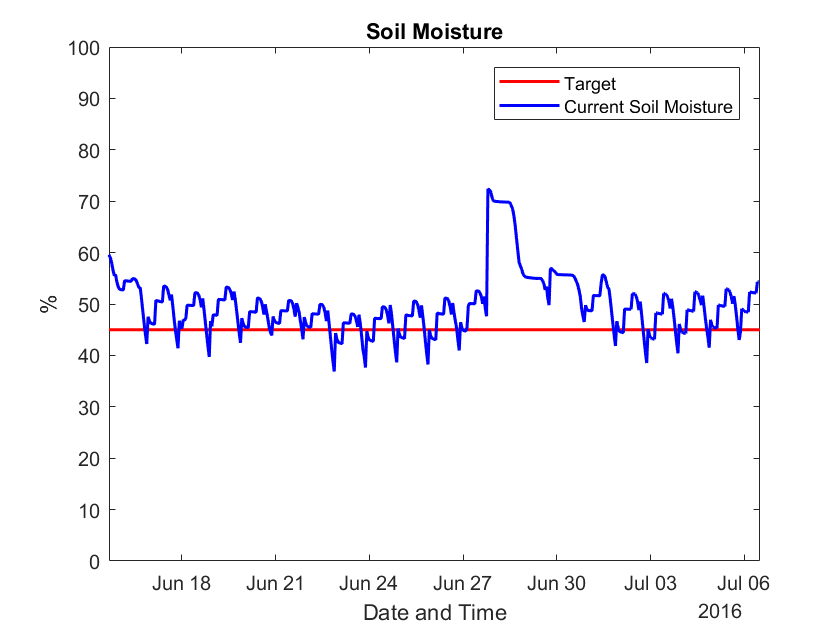
\includegraphics[width=0.9\linewidth]{images/soil_moisture.png}
	\caption{Andamento nel tempo dell'umidità del terrreno}
	\label{fig:MAD}
\end{figure}
\vspace*{-0.5 cm}
\begin{figure}[ht]
	\centering
	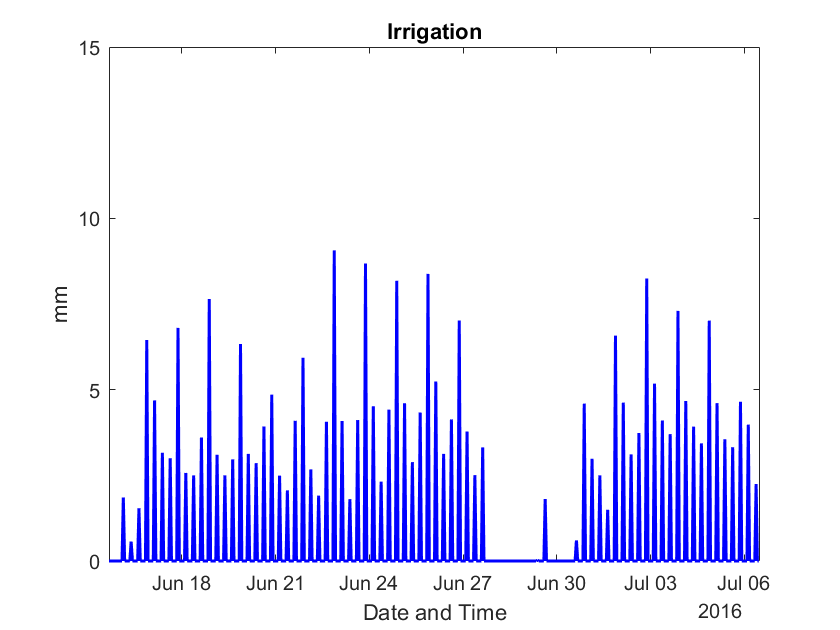
\includegraphics[width=0.9\linewidth]{images/irrigation.png}
	\caption{Andamento dell'irrigazione}
	\label{fig:MAD}
\end{figure}
\\
Notiamo nella Figure 8 come, in accordo con quanto descritto nella Figure 2, il valore di umidità resta compreso nella zona di benessere della pianta, non entrando nella regione di stress dovuta ad una eccessiva secchezza del suolo. Sono presenti però dei picchi di umidità che portano la pianta nella zona di saturazione.\\ Questi valori più elevati sono dovuti alle precipitazioni. Il sistema di irrigazione automatico ritorna a fornire acqua solamente nel momento successivo di secchezza, come si può notare della Figure 9. In questo modo si evita uno spreco di acqua, irrigando solamente quando è strettamente necessario.\\
Si nota come utilizzando questo specifico sistema di irrigazione si ottengono risultati paragonabili a quello che ci si aspetterebbe in caso di intervento umano. Viene infatti fornita acqua proporzionale a quella necessaria per mantenere la pianta ad una umidità ottima, senza mai farla ricadere nei valori di stress.\\
Interessante ora risulta il confronto con i risultati ottenuti implementando il controllore in catena chiusa.
Nelle due rappresentazioni sottostanti andiamo ad evidenziare, come nel precedente caso, l'andamento nel tempo dell'umidità del terreno (Figure 10), mentre nel grafico successivo (Figure 11) viene evidenziato la quantità d'acqua fornita tramite l'impianto di irrigazione.








%Per andare a vedere i vantaggi di una irrigazione mediante logica fuzzy, è interessante andare a valutare i valori di umidità del terreno e la quantità d'acuqa utilizzata (e soprattutto sprecato) nel caso di un approccio basato su un controllore in catena chiusa, che regola i valori di acqua da fornire in base ad un riscontro proveniente dai sensori.\\
%La logica del secondo controllore implementato era la seguente: forniva una quantità di acqua costante ogni 24 ore, dove però misurava il valore di umidità del terreno prima di irrigare, e quando trovava un valore superiore a valori tollerati, descritti dalla Figura 2, saltava il processo di irrigazione, facendo la successiva verifica 24 ore dopo.
%Possiamo paragonare l'intelligenza di questo controllore molto simile a quello che un contadino farebbe, ovvero assicurarsi della secchezza del terreno ed in base a quella provvedere alla consueta irrigazione.\\
%Poniamo anche in questo caso su grafico i valori ottenuti, relativi all'andamento nel tempo dell'umidità del suolo, e i corrispondenti valori di acqua fornita. 




%Supponiamo di andare ad usare un sistema logico che fornisce una quantità d'acqua prefissata per un determinato periodo, in una ripetizione continua nel tempo, senza ad analizzare valori esterni che possono influenzare questa decisione come temperatura e precipitazioni.\\
%Se stampiamo i grafici relativi a questo semplice controllore, tra i più presenti sul mercato, otteniamo quanto segue:\\
\begin{figure}[ht]
	\centering
	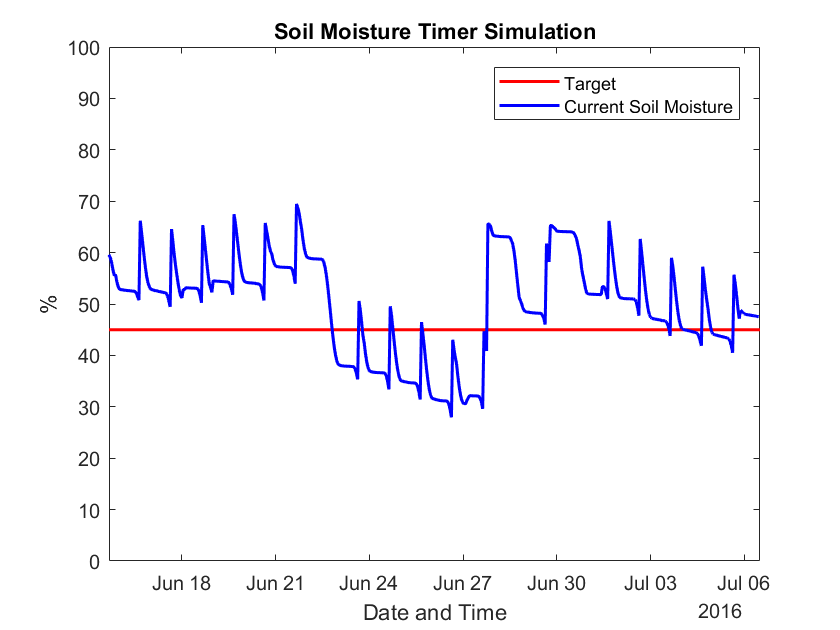
\includegraphics[width=0.9\linewidth]{images/soil_moisture_timer.png}
	\caption{Umidità nel terreno con controllore in catena chiusa}
	\label{fig:MAD}
\end{figure}
\vspace*{-0.5 cm}
\begin{figure}[ht]
	\centering
	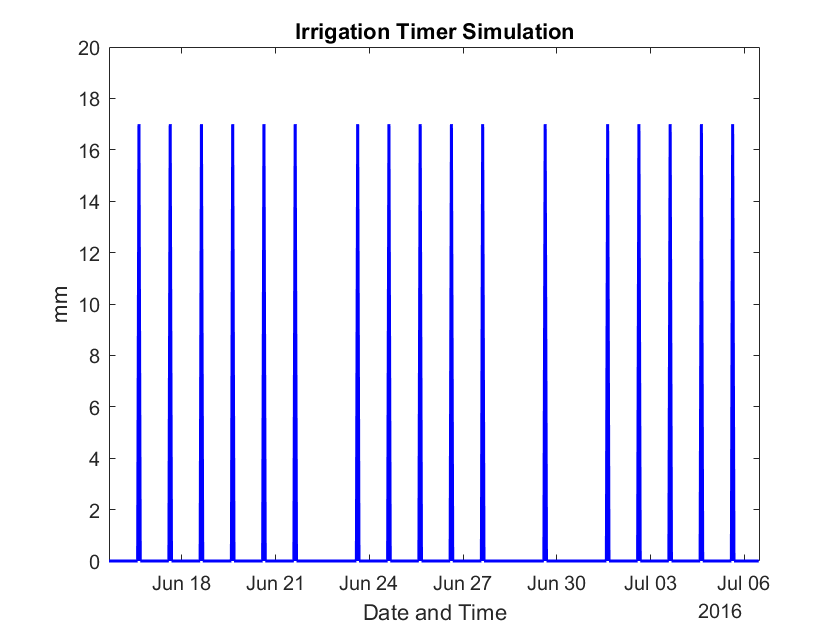
\includegraphics[width=0.9\linewidth]{images/irrigation_timer.png}
	\caption{Irrigazione con controllore in catena chiusa}
	\label{fig:MAD}
\end{figure}
Risulta evidente come l'irrigazione fornisca valori costanti d'acqua alla coltura, invece di valori graduali, ponderati alle reali necessità della pianta.\\
Si ottengo, comunque, valori di acqua irrorata paragonabili tra i due differenti sistemi automatici, ma nonostante questo si può notare dal grafico dell'umidità un andamento differente. Nella implementazione mediante logica fuzzy si ottiene un valore di umidità quasi costante all'ottimo, senza mai ricadere nel valore di secchezza e, a meno di precipitazioni, non eccedendo mai nella regione di saturazione, garantendo quindi un maggiore benessere della pianta, che ne determina la crescita ottimale.\\
Nel grafico relativo al controllore in catena chiusa troviamo un valore molto più variabile dell'umidità del terreno, infatti troviamo valori di umidità nella zona di stress della pianta, e frequentemente ci troviamo con valori superiori all'ottimo, risultati che vanno ad inficiare sullo stato di salute della pianta.



%Il confronto con i risultati ottenuti nel punto precedente evidenzia in modo netto l'effettivo guadagno in termini di acqua sprecata, ma non solo. Infatti la zona di benessere della pianta nel caso di approccio fuzzy è mantenuta nel tempo.\\
 %In caso di eventi esterni che ne modificano il valore, il valore dell'umidità rientra, dopo un certo intervallo, nei valori desiderati nel nostro modello, mentre il controllore a catena aperta è destinato ad esplodere in caso di eccessive (o nulle) precipitazioni, non potendo avere nessun riscontro dall'ambiente esterno.


%%%%%%%%%%%%%%%%%%%%%%%%%%%%%%%%%%%
\section{Conclusioni}\label{sec:conclusion}
%%%%%%%%%%%%%%%%%%%%%%%%%%%%%%%%%%%
Il modello proposto del sistema di irrigazione utilizzando la fuzzy logic ha prodotto nella sperimentazione ottimi risultati, si è dimostrato un modello molto resistente e robusto a differenti situazioni climatiche. Il modello inoltre è flessibile per differenti implementazioni, con differenti tipologie di colture e vari possibili terreni, da quelli più argillosi a sabbiosi.\\
L'obiettivo iniziale era quello di ottenere un sistema automatico che potesse emulare il comportamento umano, i grafici ottenuti mostrano appunto un andamento simile a quello che si potrebbe pensare ottenibile da piante irrigate manualmente.\\
 Un altro valore degno di nota risulta nel confronto con un altro modello di sistema automatico di irrigazione. Si ottengono, tra i due differenti modelli implementati nella trattazione, valori di acqua utilizzata durante la fase di irrigazione paragonabili. L'aspetto più vantaggioso nell'utilizzo della logica fuzzy risulta nella robustezza del sistema automatico, in grado di mantenere molto facilmente valori di umidità del suolo vicini al valore ottimo desiderato, senza effettuare grosse variazioni.\\
 Nel modello implementato con un controllore in catena chiusa troviamo invece valori di umidità che ricadono di frequente in valori di stress per la pianta, che ne compromettono la salute e la crescita ottimale.\\
Il seguente modello risulterebbe quindi una valida alternativa ai modelli di irrigazione automatica presenti attualmente in commercio .



\bibliographystyle{IEEEtran}
%\bibliography{bibi}
\bibliography{IEEEabrv,bibi}




\end{document}
